\documentclass[tikz]{standalone}
\usetikzlibrary{patterns}
\usetikzlibrary{shapes,arrows}
\usetikzlibrary{decorations.pathreplacing, positioning}
\definecolor{greengreen}{rgb}{0.0, 0.42, 0.24}
\definecolor{calpolypomonagreen}{rgb}{0.12, 0.3, 0.17}
\definecolor{forestgreen}{rgb}{0.13, 0.55, 0.13}

\begin{document}
\noindent
  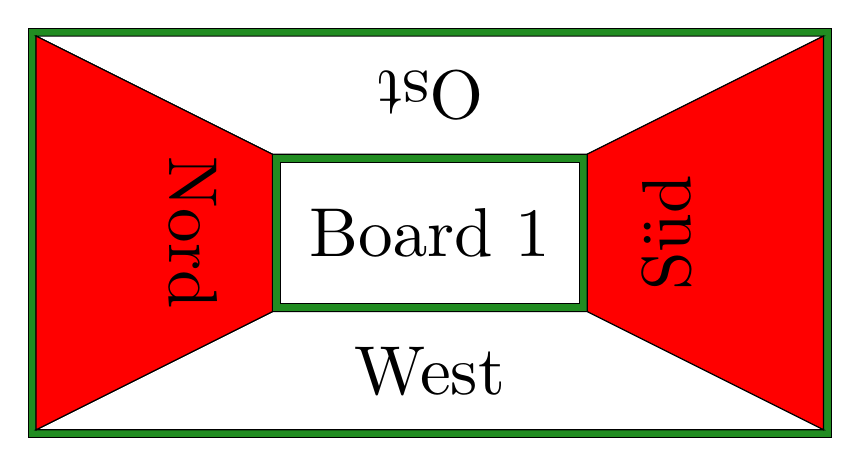
\begin{tikzpicture}

    \draw[fill=forestgreen] (-0.1,-0.1) -- (-0.1,5.1) -- (10.1, 5.1) -- (10.1, -0.1) -- cycle;
    \draw[fill=white] (0,0) -- (0,5) -- (10, 5) -- (10, 0) -- cycle;
    \draw[fill=forestgreen] (3, 1.5) -- (3,3.5) -- (7, 3.5) -- (7, 1.5) -- cycle;
    \draw[fill=white] (3.1, 1.6) -- (3.1,3.4) -- (6.9, 3.4) -- (6.9, 1.6) -- cycle;

    \node[very thick, rotate=270, scale=2.5] at (2, 2.5) {Nord};
    \node[very thick, rotate=180, scale=2.5] at (5,4.25) {Ost};
    \node[very thick, rotate=90, scale=2.5] at (8, 2.5) {Süd};
    \node[very thick, rotate=0, scale=2.5] at (5, 0.75cm) {West};


    \draw[fill=red] (0,0) -- (0,5) -- (3, 3.5) -- (3, 1.5) -- cycle;
    \draw[fill=white] (0,5) -- (10,5) -- (7, 3.5) -- (3, 3.5) -- cycle;
    \draw[fill=red] (10,5) -- (10,0) -- (7, 1.5) -- (7, 3.5) -- cycle;
    \draw[fill=white] (0,0) -- (3,1.5) -- (7, 1.5) -- (10, 0) -- cycle;

    \draw[fill=red] (0,0) -- (0,5) -- (3, 3.5) -- (3, 1.5) -- cycle;
    \draw[fill=red] (0,0) -- (0,5) -- (3, 3.5) -- (3, 1.5) -- cycle;


    \node[very thick, rotate=270, scale=2.5] at (2, 2.5) {Nord};
    \node[very thick, rotate=180, scale=2.5] at (5,4.25) {Ost};
    \node[very thick, rotate=90, scale=2.5] at (8, 2.5) {Süd};
    \node[very thick, rotate=0, scale=2.5] at (5, 0.75cm) {West};

    \node[very thick, rotate=0, scale=2.5] at (5, 2.5) {Board 1};


  \end{tikzpicture}%
\end{document}
